\begin{center}

Lecture 1

\end{center}

\section{Motivation}

\subsection{Plane Curves}

Plane curves are things like lines or circles with an orientation. The challenge is to find an quantitative characterisation of the curve at every point. This leads to the notation of curvature $\kappa$. The desired properties of curvature are:

\begin{itemize} 

\item $\kappa = 0$ for points on a straight line.
\item $\kappa \rightarrow 0$ for points on increasing circles with $r \rightarrow \infty$.
\item $\kappa \pm \frac{1}{r}$ for circles of radius $r$

\end{itemize}

$\kappa$ should be related to the change of the unit tangent vector.

\vspace{\baselineskip}

Definition: The points of minimum and maximum curvature are called vertices.

Curvature is a local concept. Figuring out the number of vertices on a whole structure is harder (Answer $\geq 4$).

\subsection{Surfaces}

Consider a torus $S$ with a point $p$ on the surface and a normal line $L$ through $p$. Slice the surface $s$ with a plane containing the normal line from $p$. The intersection is a plane curve with a curvature. Rotating this plane about the normal line $\rightarrow$ change of this curvature. We can then consider the maximum and minimum of this curvature. The product of the max and min is Gaussian curvature ($K$) and the sum is mean curvature.

$S$ plane $\implies$ $K(p) = 0$ $\forall p \in S$.

Now consider a sphere $S$ of radius $r$. If you intersect the sphere with a plane $E$ then one produces a circle which is $E \cap S$. Thus the Gaussian curvature is $K(P) = \frac{1}{r^2}$.

\subsection{Aims}

\begin{itemize}

\item Define curvature of curves and surfaces
\item Do calculations on curves and surfaces.
\item Obtain global results from local ones.
\item Look at intrinsic properties of a surface $S$ (i.e. properties related to the surface itself and not how it sits in space)

\end{itemize}

\section{Regular curves in $\mathbb{R}^n$}

Definition: A smooth curve is a smooth (infinitely many times differentiable) map $\alpha : I \rightarrow \mathbb{R}^n$ with $I \subset \mathbb{R}$ an open interval. $\alpha (I) \subset \mathbb{R}^n$ is the trace of $\alpha$

If $\alpha(u) = (\alpha_1 (u), \ldots, \alpha_n (u))$ then $\alpha_i : I \rightarrow \mathbb{R}$ is smooth.

\vspace{\baselineskip}

A tangent vector of $\alpha$ at $\alpha (u)$ is $\alpha ' (u) = (\alpha_1 ' (u), \ldots, \alpha_n ' (u)) \in \mathbb{R}^n$.

$\alpha$ is a regular curve if $\alpha ' (u) \neq 0$ $\forall u \in I$. If $\alpha$ is a regular curve, then the unit tangent vector is: $$t(u) = \frac{\alpha ' (u)}{||\alpha '(u)||}$$

If $||\alpha ' (u) || = 1$ $\forall u \in I$ then $\alpha$ is called unit speed. $\alpha$ is singular at $\alpha(u)$ if $\alpha ' (u) = 0$.

\subsubsection*{Examples}

\begin{itemize}

\item[a)] The unit circle $\alpha : \mathbb{R} \rightarrow R^2$, $\alpha (s) = (\cos s, \sin s)$. Then $\alpha ' (s) = (-\sin s, \cos s)$ $\implies$ $||\alpha ' (u) || = 1$. $\alpha$ is therefore unit speed.
\item[b)] Helix $\alpha : \mathbb{R} \rightarrow \mathbb{R}^3$ with $\alpha (u) = (\cos u, \sin u, u)$. Therefore $\alpha ' (u) = (- \sin u, \cos u, 1)$ and therefore $||\alpha ' (u) || = \sqrt{2}$
\item[c)] $\alpha : \mathbb{R} \rightarrow \mathbb{R}^3$ with $\alpha (u) = (u^3 - u, u^2 -1)$. Thus $\alpha (-1) = \alpha(1) = (0,0)$. $\alpha ' (u) = (3u^2 - 1, 2u) = 0 \Leftrightarrow 3u^2 = 1 \, \, \text{and} \, \, u = 0$ which are never satisfied. This means $\alpha$ is a regular curve but not one to one.

\end{itemize}

\begin{figure}[h]
\centering
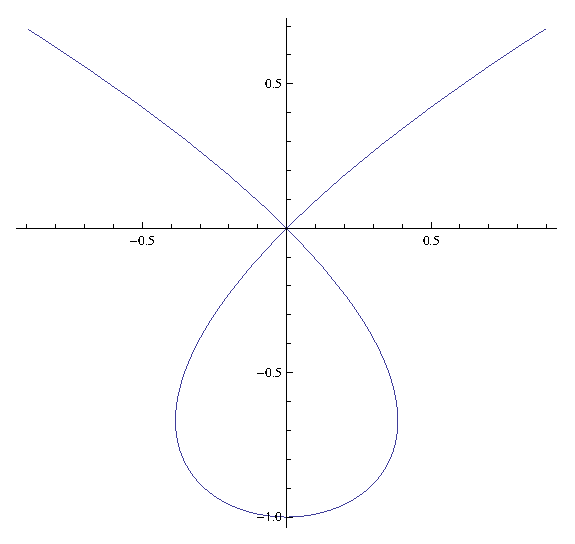
\includegraphics{img/lect1-1.eps}
\caption{A plot of the curve from example c}
\end{figure}